\section{Фрактальные антенны}

На сегодняшний день, в мире существует великое множество различных видов антенн, в зависимости от назначения и области применения они имеют различную конструкцию. Тип антенн, о котором пойдёт речь в этом разделе, появился сравнительно недавно, и принципиально отличается от известных, стандартных и общепринятых решений. К тому же им пророчат большое будущее. Речь пойдет, о так называемых фрактальных антенных. Фрактальная антенна – это антенна, активная часть которой имеет вид самоподобной кривой или какой либо другой подобно делящейся или состоящей из подобных сегментов фигуры. Что бы иметь более понятное представление о такой форме, нужно обратиться к фрактальной геометрии.

Фрактальная геометрия утверждает, что практически любые природные формы с математической точки зрения являются фракталами. Фрактал – от латинского: Fractus – сломанный, разбитый. Получить фрактал можно разделив фигуру на всё более мелкие объекты, деление может осуществляться бесконечно. Таким образом, любая из полученных фигур будет делиться на подобные, и в свою очередь являться частью такой же фигуры.

\begin{figure}[H]
    \centering
    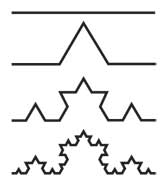
\includegraphics{img/fractals.jpeg}
    \caption{Примеры фракталов}
    \label{fig:fractals}
\end{figure}


Впервые на практике для антенн эти принципы применил в 90-е года XX века американский инженер Натан Коэл. Коэл, задумавшись о принципах фрактальной геометрии, взял обычную медную проволоку и придал ей форму самоподобной ломанной кривой, после чего, подключив её к своему радиоприёмнику, поразился на сколько хорошо она работает. Продолжая развивать это направление в построении антенн выяснилось, что при помощи фракталов можно значительно уменьшить размеры конструкции, и расширить полосу рабочих частот, т. е. можно создать широкополосную антенну. Последующие  математические расчеты показали, что действительно широкополосная антенна, диапазон частот которой может охватить весь радиоволновой спектр, должна иметь фрактальную форму.

Дальнейшие исследования в этой области привели к широкому практическому использованию фрактальных антенн в мобильных устройствах. Их компактность и широкополосные свойства сделали их незаменимыми в беспроводной связи, в Bluetooch, Wi-Fi и GSM стандартах. Таким образом, в одном гаджете, например, в мобильном телефоне, смартфоне, КПК, удалось разместить все эти устройства. Многие микроволновые устройства тоже используют фрактальные антенны. Отличная работа фрактальных антенн в телевизионном диапазоне так же была отмечена. Отсутствием широкого применения фрактальной конструкции таких антенн в производстве, объясняется тем, что патентом на производство и внедрение фрактальных систем в антенной промышленности владеет весьма  ограниченное количество компаний

Первой конструкцией фрактальной антенны с наиболее
полно изученными электромагнитными и направленными
свойствами стала антенна на основе префрактальной кривой
Коха. При построении линии Коха исходный отрезок длиной
$z$, именуемый инициатором фрактала, делится на три равные
части. Центральный участок заменяют равносторонним треугольником со стороной $\frac{z}{3}$. В результате образуется ломаная,
состоящая из четырех звеньев длиной $\frac{z}{3}$ каждый (рис. \ref{fig:koch}).

\begin{figure}[H]
    \centering
    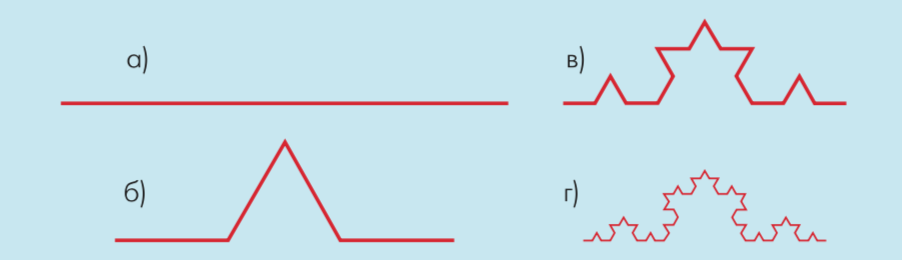
\includegraphics[width=.9\textwidth]{img/koch.png}
    \caption{построение кривой коха: а) первая, б) вторая, в) третья и г) четвертая итерации}
    \label{fig:koch}
\end{figure}

Этот процесс повторяется для каждого отдельного сегмента
ломаной линии: во второй итерации на отрезках $\frac{z}{3}$ строятся треугольники со сторонами $\frac{z}{9}$, на них – треугольники со
сторонами $\frac{z}{27}$ (третья итерация) и т.д. Предельная кривая и 
есть кривая Коха. Каждый шаг синтеза увеличивает длину результирующей кривой в соответствии с выражением


\[
    L = z  \left( \frac{4}{3}\right)^n
\]

где $n$ – число итераций, $z$ – высота образующего шаблона (длина исходного отрезка).

Этот эффект миниатюризации антенн является существенным лишь при пяти-шести первых итерациях фрактала.

Строго говоря, в антенных решениях используются не подлинные фракталы, а лишь несколько первых их итерационных форм, получивших в геометрии название кривых, заполняющих пространство (Space-Filling Curves, SFC) или плоскость (Plane-Filling Curves, PFC). Реже используется термин "префракталы". Все эти понятия применительно к антенным конструкциям могут употребляться как синонимы. Такова исторически сложившаяся терминология теории фрактальных антенн, хотя она и не соответствует принятым математическим определениям.

SFC могут применяться в качестве шаблонов для изготовления монополей и плеч диполей, формирования топологии печатных антенн, частотно-селективных поверхностей (Frequency Selection Surfaces, FSS) или обечаек зеркальных рефлекторов, построения контуров рамочных антенн и профилей апертуры рупоров, а также фрезеровки пазов в щелевых антеннах. В англоязычной литературе соответствующие антенны нередко называют "space-filling antenna" (SFA) (антенны, заполняющие пространство).

В случае проволочных антенн самопересечение SFC допускается только в начальном (или конечном) пункте. Иначе говоря, фрактальная линия может иметь вид замкнутого контура, но ни одна из ее частей не может быть замкнутым фрагментом. Отсутствие точек самоконтакта в SFC-объектах позволяет говорить о них как о "самоизбегающих" кривых. Отсюда, кстати, происходит еще одно название этих ломаных линий – FASS-кривые (space-Filling self-Avoidance Simplicity Similarity – самоуклоняющиеся кривые подобных сегментов, заполняющих пространство).

Существует и другое ограничение всех типов фрактальных антенн: сегменты используемых в них SFC-линий должны быть короче одной десятой рабочей длины волны антенны в свободном пространстве. При этом желательно, чтобы общее число связанных SFC-сегментов в антенных топологиях превышало 10.

Экспериментальные данные, полученные специалистами компании Cushcraft для кривой Коха, четырех итераций меандра и спиральной антенны, позволяют сопоставить электрические свойства антенны Коха с другими излучателями с периодической структурой. Все сопоставленные излучатели обладали многочастотными свойствами, что проявилось в наличии периодических резонансов на графиках импедансов. Однако для многодиапазонных приложений более всего пригоден фрактал Коха, у которого с ростом частоты пиковые значения реактивных и активных сопротивлений уменьшаются, тогда как у меандра и спирали они возрастают.

В целом следует отметить, что теоретически представить механизм взаимодействия фрактальной приемной антенны и падающих на нее электромагнитных волн сложно из-за отсутствия аналитического описания волновых процессов в проводнике со сложной топологией. В такой ситуации основные параметры фрактальных антенн целесообразно определять путем математического моделирования. Численному исследованию электромагнитных процессов, протекающих во фрактальных антеннах и при их взаимодействии с предметами окружающей среды, посвящено достаточно много работ. Их подробный обзор и анализ выходит за рамки данной работы. Общий недостаток всех известных публикаций по результатам исследований фрактальных антенн – отсутствие указаний на статистическую обработку результатов экспериментов. В частности, в них не приводятся сведения о доверительных интервалах для измеренных параметров, что не позволяет судить о точности полученных в итоге эмпирических соотношений. В целом же, статистическая теория фрактальных антенн при расчете их численными методами пока еще ждет своих разработчиков.

Пример построения первой самоподобной фрактальной кривой продемонстрировал в 1890 году итальянский математик Джузеппе Пеано (Peano). Предложенная им линия в пределе полностью заполняет квадрат, обегая все его точки (рис. \ref{fig:peano1}). В дальнейшем были найдены и другие подобные объекты, получившие по имени первооткрывателя их семейства обобщающее название "кривые Пеано". Правда, вследствие чисто аналитического описания кривой, предложенного Пеано, возникла некоторая путаница в классификации SFС-линий. На самом деле наименование "кривые Пеано" следовало бы давать лишь оригинальным кривым, построение которых соответствует аналитике, опубликованной Пеано (рис. \ref{fig:peano2}). Поэтому для конкретизации рассматриваемых объектов антенной техники при описании той или иной формы фрактальной антенны следует, по возможности, упоминать и имена авторов, предложивших соответствующую модификацию SFC. Это тем более важно, что согласно подсчетам, число известных разновидностей SFC приближается к трем сотням, причем эта цифра не является предельной.

\begin{figure}[H]
    \centering
    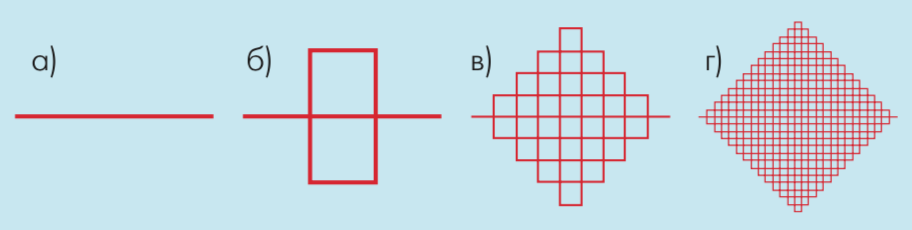
\includegraphics[width=.9\textwidth]{img/peano1.png}
    \caption{Итерации кривой пеано: а) исходная линия, б) первая, в) вторая и г) третья итерации}
    \label{fig:peano1}
\end{figure}

Следует отметить, что кривая Пеано (см. рис. \ref{fig:peano1}) в исходном виде вполне пригодна для изготовления щелей в стенках волновода, печатных и других апертурных фрактальных антенн, но не приемлема для построения проволочной антенны, поскольку имеет соприкасающиеся участки. Поэтому специалистами компании Fractus была предложена ее модификация, получившая название "Peanodec" (рис. \ref{fig:peano2})

\begin{figure}[H]
    \centering
    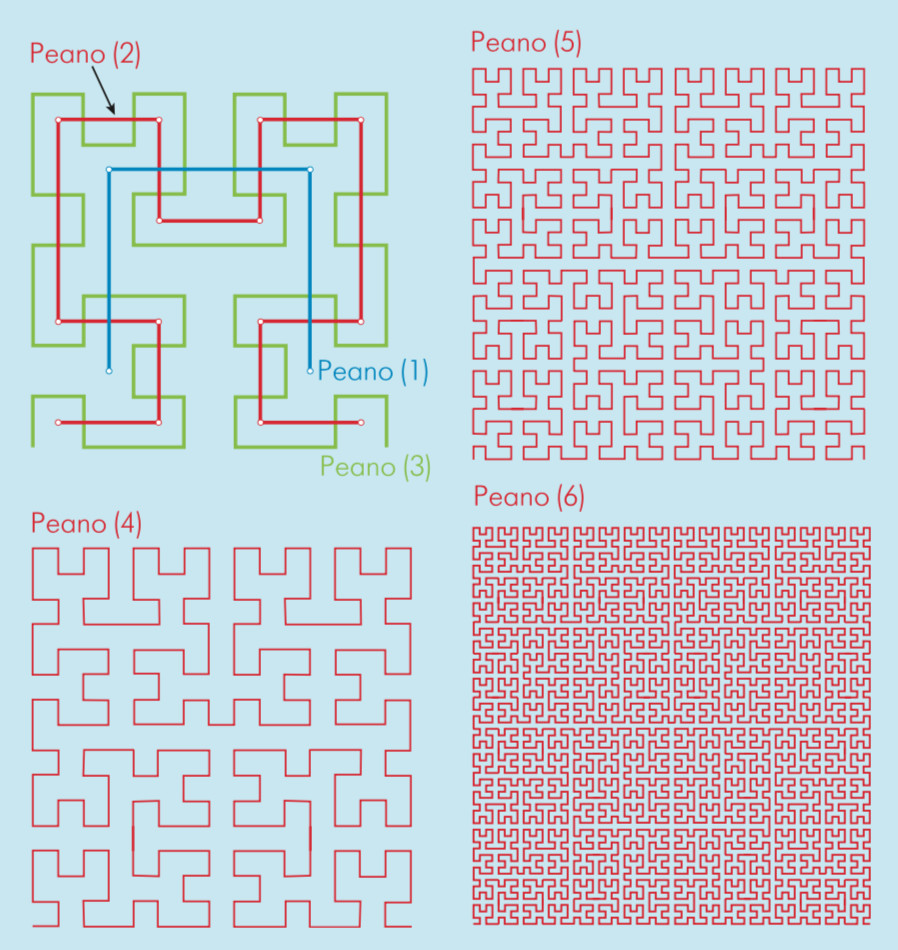
\includegraphics[width=.9\textwidth]{img/peano2.png}
    \caption{Итерации ломаной, предложенной Гильбертом в 1891 году [8]. нередко трактуется как рекурсивная кривая пеано [15]}
    \label{fig:peano2}
\end{figure}

Представленная на рис.\ref{fig:koch} антенна по фракталу Коха – лишь один из вариантов, реализуемый при использовании равностороннего инициирующего треугольника рекурсии, т.е. угол $\theta$ при его основании (indentation angle или "угол углубления") равен 60°. Такой вариант фрактала Коха принято называть стандартным. Вполне естественно задаться вопросом, можно ли использовать модификации фрактала с иными значениями этого угла. Утвердительный и обстоятельный ответ на данный вопрос содержится в работе ученого Пенсильванского университета К.Дж.Виной (K.J.Vinoy). Виной предложил рассматривать угол при основании инициирующего треугольника в качестве параметра, характеризующего антенную конструкцию. Изменяя этот угол, можно получать аналогичные рекурсивные кривые разной размерности (рис. \ref{fig:koch2}).

\begin{figure}[H]
    \centering
    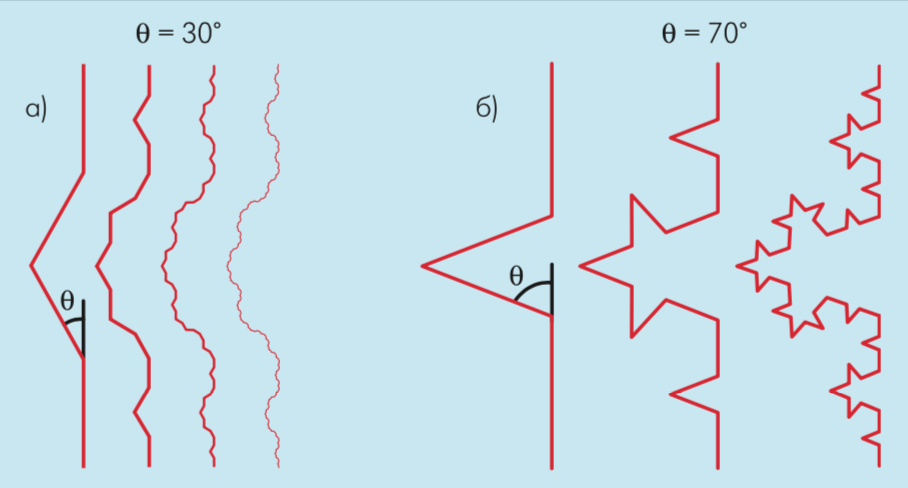
\includegraphics[width=.9\textwidth]{img/koch2.png}
    \caption{Построение кривой коха с углом θ а) 30° и б) 70° при основании треугольника в генераторе фрактала}
    \label{fig:koch2}
\end{figure}


Кривые сохраняют свойство самоподобия, однако результирующая длина линии может быть различной, что влияет на характеристики антенны. Виной первым исследовал корреляцию между свойствами антенны и размерностью обобщенного фрактала Коха $D$, определяемой в общем случае зависимостью:

\[
L_{n,\theta} = \left( \frac{2}{1+\cos \theta}\right)^n \cdot L_0,
\]

где $L_0$– длина линейного диполя, расстояние между концами которого то же, что и у ломаной Коха, $n$ – номер итерации. Переход от θ = 60° к θ = 80° на шестой итерации позволяет увеличить общую длину префрактала более чем в четыре раза.


Как и следовало ожидать, между рекурсивной размерностью и такими свойствами антенны, как первичная резонансная частота, внутреннее сопротивление на резонансе и многодиапазонные характеристики, существует прямая связь.

Перспективное применение антенн с топологией Коха – MIMO-системы связи (системы связи со многими входами и выходами). Для миниатюризации антенных решеток абонентских терминалов в таких средствах коммуникации специалисты Лаборатории электромагнетизма Университета Патраса (Греция) предложили фрактальное подобие перевернутой L-антенны (ILA). Суть идеи сводится к изгибу вибратора Коха на 90° в точке, делящей его на сегменты с соотношением длин 2:1. Для мобильных средств связи с частотой несущей $\sim$2,4 Гц габариты такой антенны в печатном исполнении составляют 12,33×10,16 мм ($\sim$λ/10×λ/12), полоса пропускания – $\sim$20\% и КПД – 93\%. Диаграмма направленности по азимуту почти равномерна, коэффициент усиления в пересчете ко входу фидера составляет $\sim$3,4 дБ. Правда, как отмечено в источнике, работа таких печатных элементов в составе решетки (рис. \ref{fig:two-d}) сопровождается снижением их КПД по сравнению с единичным элементом. Так, на частоте 2,4 ГГц КПД согнутого на 90° монополя Коха снижается с 93 до 72\%, а на частоте 5,2 ГГц – с 90 до 80\%. Несколько лучше обстоит дело с взаимным влиянием антенн высокочастотной полосы: на частоте 5,25 ГГц развязка между элементами, образующими центральную пару антенн, составляет 10 дБ. Что касается взаимного влияния в паре соседних разнодиапазонных элементов, то в зависимости от частоты сигнала развязка изменяется от 11 дБ (на 2,45 ГГц) до 15 дБ (на частоте 5,25 ГГц). Причина ухудшения эффективности работы антенн – взаимное влияние печатных элементов.

\begin{figure}[H]
    \centering
    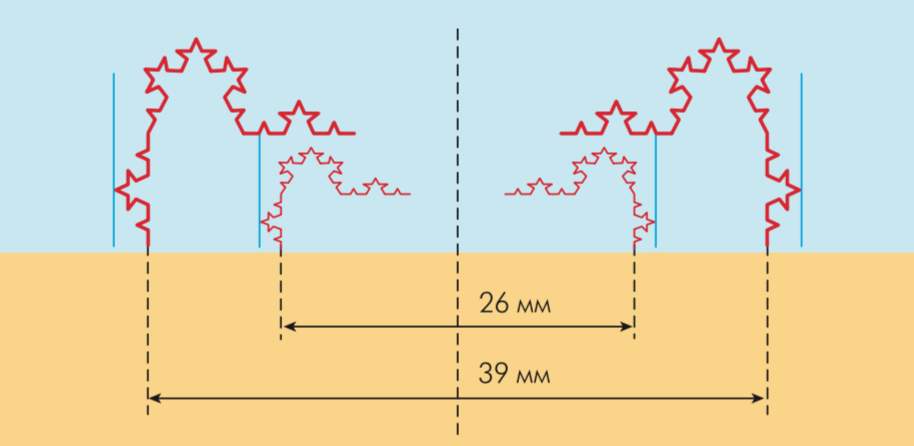
\includegraphics[width=.9\textwidth]{img/two-d.png}
    \caption{Пример двухдиапазонной (2,45 и 5,25 ГГц) антенной решетки}
    \label{fig:two-d}
\end{figure}


Таким образом, возможность выбора множества разнообразных параметров антенной системы на основе ломаной Коха позволяет при проектировании удовлетворять различные требования, предъявляемые к значению внутреннего сопротивления и распределению резонансных частот. Однако, поскольку взаимозависимость рекурсивной размерности и характеристик антенны может быть получена только для определенной геометрии, справедливость рассмотренных свойств для других рекурсивных конфигураций нуждается в дополнительном исследовании.



